\subsection{Methods}
We will use a convolutional autoencoder, i.e. an autoencoder which uses convolutional layers, which are particularly useful in the case of images.
An autoencoder is formed by two main structures:
\begin{itemize}
    \item An Encoder, which takes the input and transforms it in a limited series of parameters $\{\xi_i\}_{i=1,\dots, N}$ which captures the characteristics of that input, and we 
        call the space where these parameters lives, i.e. $\mathbb{R}^N$, encoded space. Its architecture is shown in Figure \ref{fig:enc_arch};
    \item A Decoder, which has the same structure of the encoder but mirrored. It transforms points in the encoded space back into samples of the same type of the input.
        Its architecture is shown in Figure \ref{fig:dec_arch}.
\end{itemize}
To avoid vanishing problems in the gradient we will use a rectified linear unit (ReLU) as activation function.
\begin{figure}[h]
    \centering
    \begin{minipage}[t]{0.48\textwidth}
        \centering
        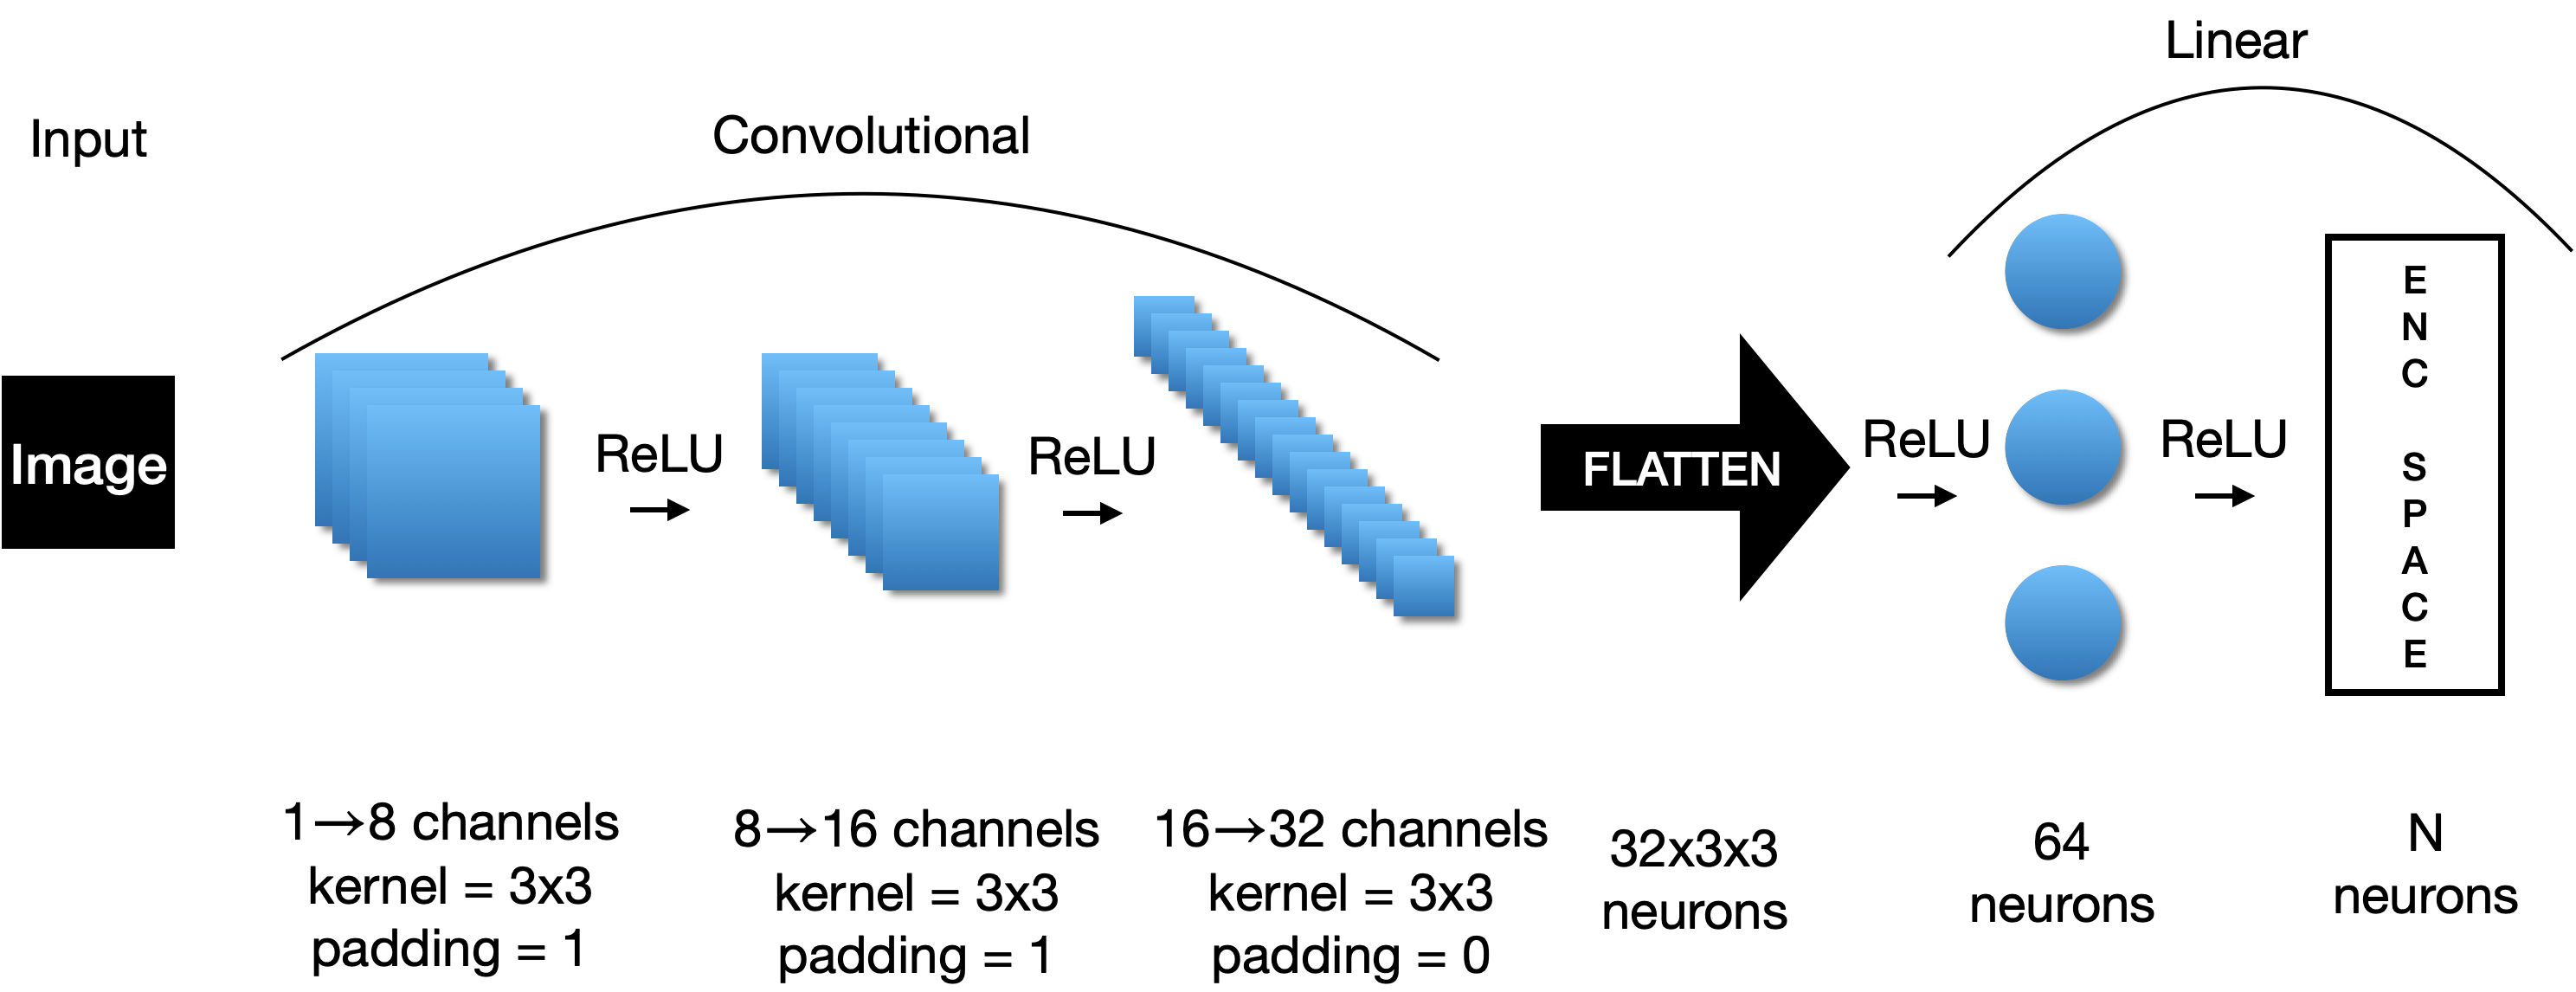
\includegraphics[width=0.98\textwidth]{Images/Encoder.png}
        \caption{Architecture of the Encoder structure of the Autoencoder.}
        \label{fig:enc_arch}
    \end{minipage}\hfill
    \begin{minipage}[t]{0.48\textwidth}
        \centering
        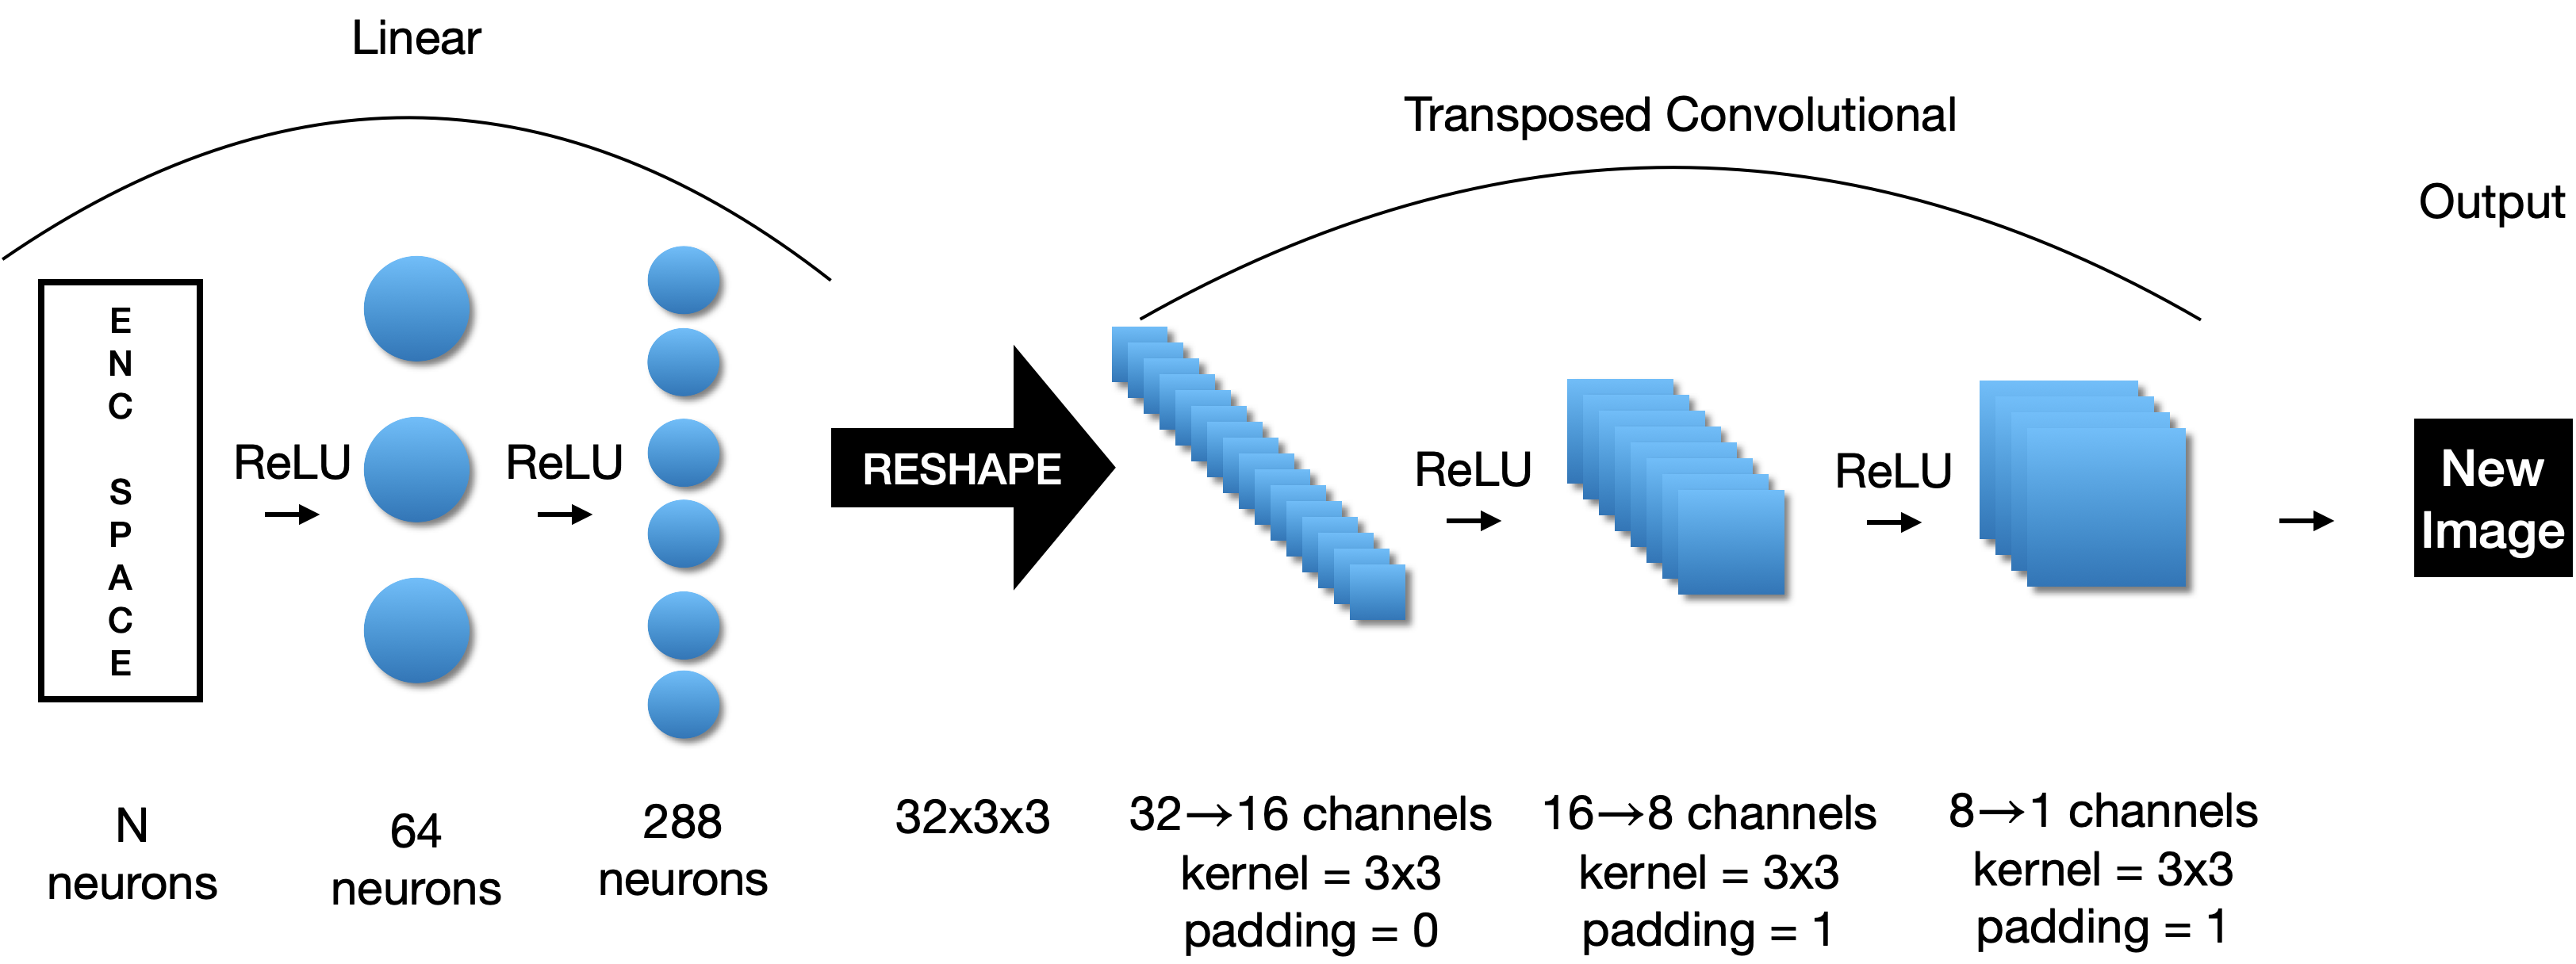
\includegraphics[width=0.98\textwidth]{Images/Decoder.png}
        \caption{Architecture of the Decoder structure of the Autoencoder.}
        \label{fig:dec_arch}
    \end{minipage}
\end{figure}
We will implement a regularization procedure, to better generalize outside of the training set. We choose to use the L2 regularization, which consists of adding a penalty 
in the loss proportional to the 2-norm of the parameters, i.e. weights and biases. In pytorch this method is enabled not in the loss
function but in the optimizer, using the \lstinline{weight_decay} keyword.

We will try two different optimizers:
\begin{enumerate}
    \item The stochastic gradient descent with momentum, which is the really basic algorithm for optimization.
        The addition of the momentum, i.e. the memory of previous steps, really helps to go out of local minima and speeds up convergence;
    \item the Adam algorithm, adaptive moment estimator, a more advanced algorithm that uses estimations of first and second 
        moments  of the gradient to adapt the learning rate of each weight of the neural network.
\end{enumerate}

To optimize the hyperparameters of the network we will use the Optuna framework\cite{optuna_2019}, which consists of a python library which performs a bayesian optimization of the 
hyperparameters. Bayesian optimization basically infere the next best parameters based on the previous tests. It is a more advanced and better approach then grid/random search, 
since it "learns" from previous tests, while the grid/random search are completely memoryless. Indeed, we already shown of being able of implementing a cross validation setup in 
Homework 1, and since it has been proved that the Cross Validation is an approximation of bayesian optimization\cite{fong2020marginal} we will not implement it in this homework.
Furthermore, the MNIST dataset is quite exhaustive with respect to its statistical variability, and a cross validation technique is not necessary to avoid overfitting.
We will also make use of an early stopping, i.e. we will prune  trials that do not improve their performances.
The hyperparameters that we will optimize are:
\begin{itemize}
    \item The weight of the L2 regularization;
    \item The optimizer, between the Adam and the SGD with momentum;
    \item The learning rate of the optimizer;
    \item The encoded space dimension;
\end{itemize}
We will indeed keep the dimension of the encoded space small, since we want to compress as much as possible the informations in the image.

To quantify the performances of the autoencoder we will use the mean square error loss between the original image and the one reconstructed by the network.

\subsection{Results}
The hyperparameter search started from a very lucky point, as we can see from Figure \ref{fig:opt}. 
We can observe the reconstruction loss in Figure \ref{fig:losses}, and we see that the loss converges quickly to low values. On Figure \ref{fig:hyper}
we can observe instead all the different combination of hyperparameters with their validation loss. It is really clear that the Adam is the best 
optimizer for this task. The regularization has a very low value, and the learning rate is really near the higher bound. This might suggest that a new 
search should have been implemented, increasing the higher bound on the learning rate. What is really interesting is, however, that the encoded space 
dimension $N=9$ is the one performing better. This suggests that $N=9$ is a sufficient dimension, and further enlargements are not needed.

We trained again a network using $100$ epochs and we present in Figure \ref{fig:rec} examples of the reconstructions on the test set, with a test loss
of $0.0164$.